\chapter{鲁棒性}
\label{chap:trust-robustness}

一个邮件分类器通过了旧月份的测试，到了新月份却频繁误拦正常邮件。要定位问题，先得看这一个月里究竟是什么变了。一种变化发生在测量环节：同一封邮件换了压缩方式，或网关的 OCR 版本升级，模型读到的像素、字符与旧版本不同，但邮件是不是垃圾邮件并没有改变。另一种变化发生在规律本身：正常业务也开始采用过去只在垃圾邮件里出现的模板，于是“带某个页脚就是垃圾邮件”这条旧规律不再成立。前者只要求模型对同一封信的不同呈现保持判断，后者则要求模型识别并学习已经改变的规律。两类问题需要的证据和补救完全不同，所以谈“模型稳不稳”之前，必须先回答：部署时究竟要求它承受哪些变化。

\term{鲁棒性}（robustness）讨论的就是这个问题：在事先规定的变化范围内，模型能否继续完成任务。它不是一句笼统的“抗干扰能力强”。一条鲁棒性主张要写清三件事：变化的对象（输入测量、群体比例，还是特征与标签的关系）、变化的范围（允许多大噪声、哪些环境），以及衡量表现的指标和最低标准。缺了任何一项，“稳健”就没有确定的评价对象——对压缩鲁棒、对模板更换鲁棒和对全新诈骗类型鲁棒，是三个完全不同的承诺。在第~\ref{chap:trust-foundations}章的三层框架中，这份声明属于要求层。

模型并不总能在变化中保持准确。变化超出了声明范围，或者现有数据不足以判断模型是否仍然可靠时，部署系统还应能识别异常输入、拒绝自动处理或回退到人工，把损害控制住。这一层能力称为\term{变化应对能力}（resilience to change）。两者评价的对象不同：鲁棒性问“模型在变化中还准不准”，变化应对问“模型不可靠时系统会不会闯祸”。

这两个问题都承接上一章。上一章的校准、覆盖和风险保证都建立在“校准数据与未来输入满足某种关系”（如可交换、独立同分布）之上；关系一旦改变，这些主张就可能失效。本章先界定变化范围并分析模型为什么会在变化中出错（第~\ref{sec:robustness-fragility}节），再分别检验变化后的风险、邻域内的稳定性和系统的止损能力（第~\ref{sec:robustness-evaluation}节），最后按诊断出的失效机制选择增强措施（第~\ref{sec:robustness-enhancement}节）。第~\ref{chap:transfer-learning-theory}章给出了变化下“哪些规律可学”的条件，本章把这些条件接到具体的检验与改进方法上。允许的变化也可能由对手主动寻找；本章只按“允许集合加损失”的抽象形式讨论，攻击者的权限、资源和损害路径留到第~\ref{chap:trust-security}章。

\section{模型的鲁棒性}
\label{sec:robustness-fragility}

要系统地回答“模型在变化中表现如何”，先把两件事分开。第一是变化范围：部署时允许哪些输入或环境发生变化，这决定了应该测试什么。第二是失效机制：模型为什么会在这些变化中出错，这决定了应该怎样补救。二者不是一一对应的：同一种变化（如附件压缩）可能因不同机制导致失败，同一条脆弱规律（如依赖页脚）也可能被多种变化暴露。

\subsection{变化范围与性能要求}
\label{sec:robustness-change-scope}

先考虑最简单的一类变化：邮件的正确标签不变，只是它在模型眼里的呈现可以改变。固定参考邮件总体$\mathcal P$（旧月份邮件及其标签的联合分布）与预测器$f$。对每封邮件$\bm{x}$，任务规定一个非空的\emph{允许集合}$U(\bm{x})$：它包含原输入$\bm{x}$本身，集合中的每个变体$\bm{x}'$都代表同一封邮件，正确标签仍是$y$。允许集合由任务给出：对图像可以是“像素改动的$\ell_2$范数不超过某个半径”，对文本可以是“同义改写或 OCR 误识的可能形式”，对邮件可以是“允许的压缩和编码差异”。

接下来要把“在允许集合内都不出错”写成一个可以比较的数。设损失$\ell(f(\bm{x}),y)$越大表示预测越差。对一封邮件，先在它的允许集合里找最差的变体，即对损失取上确界（集合中损失的最小上界；集合有限时就是最大值）；再对参考总体求平均：
\begin{equation}
 R_{\mathrm{pert}}(f)
 =\mathbb E_{(\bm{x},y)\sim\mathcal P}
   \left[\sup_{\bm{x}'\in U(\bm{x})}
   \ell(f(\bm{x}'),y)\right].
 \label{eq:robustness-perturbation-risk}
\end{equation}
用零一损失时，方括号内的量只取0或1：只要允许集合里存在一个分错的变体，它就等于1。于是$R_{\mathrm{pert}}$是“至少有一个变体被分错”的邮件所占比例。为什么不对扰动再取一次平均？随机抽样扰动只描述“平均加噪后错多少”，可能漏掉少数改动很小却让模型翻转的点；上确界则对应一个全称要求——集合里的每一个变体都必须分对。预设容限$\rho_{\mathrm{pert}}$后，可以要求$R_{\mathrm{pert}}(f)\leq\rho_{\mathrm{pert}}$。

哪些变化可以进入$U$由任务决定。像素噪声、等义改写、测量误差都可以；删除否定词虽然只动几个字符，却改变了邮件含义和标签，就不能要求模型对它保持原输出。

式~\eqref{eq:robustness-perturbation-risk}还有一个局限：外层总体$\mathcal P$始终没变，变化只发生在单封邮件的邻域内。新月份带来的往往不是这种局部改动，而是邮件构成乃至特征与标签的关系都变了。为描述这种变化，引入环境集合$\mathcal E$：每个环境$e\in\mathcal E$对应一个数据分布$\mathcal P_e$，参考环境记为$0\in\mathcal E$且$\mathcal P_0=\mathcal P$，模型在环境$e$中的风险为$R_e(f)=\mathbb E_{(\bm{x},y)\sim\mathcal P_e}\ell(f(\bm{x}),y)$。环境集合声明允许改变什么：各类邮件的比例、标签比例、输入的边缘分布，还是给定输入后的标签规律，具体类型见第~\ref{sec:distribution-shift}节。

在环境集合上可以提出两种要求：约束最坏环境的风险水平$\sup_{e\in\mathcal E}R_e(f)\leq\rho$，或约束相对参考环境最多恶化多少$\sup_{e\in\mathcal E}[R_e(f)-R_0(f)]\leq\delta$。前者问“最差时有多差”，后者问“变化让它变差了多少”。两个数要一起报告：一个本来就很差的模型在新环境中可能恶化很小，风险水平却始终不可接受。局部邻域上的保证通常也推不出这两个环境层面的保证，因为它们约束的是不同的分布。

\begin{example}[总体表现掩盖群体脆弱性]
\label{ex:robustness-mixture}
构造一个旧环境：99\%的邮件使用常见模板，模型在这类邮件上的错误率只有1\%；另有1\%的邮件使用少见模板，模型对它们的错误率高达50\%。按各组所占比例加权，总体错误率只有
\[0.99\times0.01+0.01\times0.5=0.0149\text{，}\]
即1.49\%，看起来相当好。到了新环境，模型本身和它在每一类邮件上的表现都没有变化，只是少见模板的比例从1\%提高到30\%，总体错误率便变成
\[0.70\times0.01+0.30\times0.5=0.157\text{，}\]
即15.7\%。按前面的两种要求读，新环境的风险水平是15.7\%，相对旧环境恶化了约14.2个百分点。模型参数和组内表现都没有变，仅仅是群体比例改变，就足以让总体表现大幅退化；只看旧环境的一个总体平均数，会把这种脆弱性掩盖掉。
\end{example}

图~\ref{fig:trust-robust-neighborhood}把后面检验部分要用到的两种动作画在一起。允许集合中的一个错误变体，就足以反驳“这封邮件在整个邻域都正确”的全称主张；但要对总体容限下结论，还要按参考样本的抽样方式把逐样本结果聚合起来。反过来，要证明整个邻域都稳定，需要一种覆盖邻域中每一个点的认证依据，抽几个点试试是不够的。搜索反例、总体估计和邻域认证是三种不同对象，第~\ref{sec:robustness-evaluation}节分别展开。

\begin{figure*}[!htb]
  \centering
  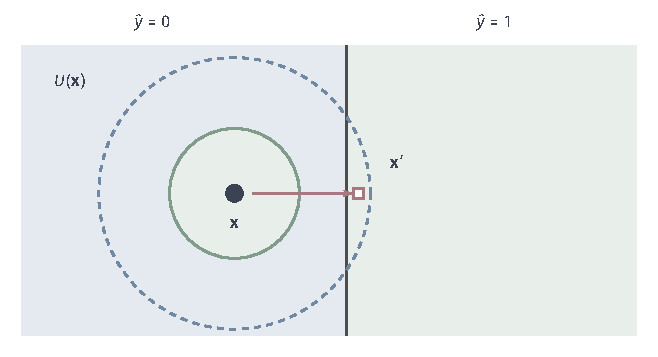
\includegraphics[width=111.404mm]{figures/06-foundations/03-trustworthiness/tikz/trust-robust-neighborhood/figure.pdf}
  \caption{虚线圈为允许集合$U(\bm x)$，内圈为已认证稳定范围，方点$\bm x^{\prime}$在允许集合中跨越决策边界。尺寸仅示意集合关系，未取自随机平滑实验。搜索无反例尚未认证全允许范围。}
  \label{fig:trust-robust-neighborhood}
\end{figure*}

\subsection{失效机制与信息缺口}
\label{sec:robustness-failure-mechanisms}

允许范围只告诉我们“测什么”，还没有解释“为什么会出错”。失效机制不同，补救需要的信息也不同。本章主要涉及三种机制。第一，决策边界离输入太近，输入轻微改动就越过边界，预测随之翻转。第二，原本错误率就高的群体在新环境中占比变大，平均风险被抬高；示例~\ref{ex:robustness-mixture}就是这种情形，它没有制造任何新的组内错误，只是给本来就困难的样本增加了权重。第三，特征与标签之间的联系本身改变，旧规则不再成立。

这三种机制都假定记录本身可信，应与标注错误、测量异常等数据质量问题分开。后者应先核查记录的来源和含义，再决定修正数据、补充观测，还是采用适合该类污染的稳健损失或估计方法。不能只凭残差大就把合法的困难样本当作脏数据，修数据与改估计方法也不是只能二选一。

第三种机制最隐蔽，要从训练目标本身理解。如果训练只最小化当前样本上的分类损失，目标函数奖励的只是“在训练条件下把这批样本分对”，并不区分模型使用的关系能不能迁移到新条件。设想垃圾邮件长期带一个固定页脚，模型记住“有这个页脚就判垃圾邮件”，在旧月份可以稳定答对；一旦正常邮件也开始带这个页脚，这条依据立刻失效。\term{捷径学习}（shortcut learning）指的就是这种现象：模型学到一条在训练条件下有效、却不足以支撑预期迁移的规则。Geirhos 等用图像模型对背景和纹理的依赖系统说明了这类问题，并强调捷径的认定必须结合数据和评价条件，不能只凭特征“看起来不本质”下判断\scite{geirhos2020shortcut}。

页脚是不是捷径，取决于鲁棒性要求是否包含“页脚改变而类别保持”这种变化。在业务关系长期稳定的场景里，页脚完全可能是合法且高效的判别依据。判断时还要避免两种直觉错误：直观易读的特征未必稳定（发件人显示名也可以被伪造），高维、抽象的特征也未必是捷径（它们可能承载因果信息）。可靠的判定方式是实际改变这层关系，观察预测是否跟着出错。

一个人为对照可以说明为什么随机留出检验不出捷径。设垃圾邮件中90\%使用模板甲，正常邮件中90\%使用模板乙，那么规则“模板甲判垃圾、模板乙判正常”在每一类上都答对90\%，总准确率也是90\%。按原比例随机划分训练集和测试集，测试集保持同样的比例，这条规则在测试集上仍有90\%的准确率，问题暴露不出来。如果测试时让两种模板在两类中各占一半（模板与标签脱钩），同一条规则在每一类上都只答对一半，准确率降到50\%，与抛硬币相当。这个对照不说明所有模型都会去学模板；它说明随机留出只检验了同一分布内的泛化，没有检验“模板改变后模型是否仍靠内容判断”。

如果现有环境里模板与标签始终同向出现，数据中就没有排除捷径所需的信息，任何模型选择方法都无法凭空判断哪条关系更可靠。增加环境多样性才可能把它暴露出来，但多样性必须对准目标变化：同一模板的近重复邮件再多，也不增加对“模板脱钩”情形的覆盖。更极端地，若两种不同的标签规律都与现有资料完全相容，却在目标域给出不同预测，那么无论模型多复杂、无标签适应多积极，都补不出数据中不存在的信息；定理~\ref{thm:transfer-nonidentifiability}给出的正是这类不可识别边界。

最后，“输出不变”不是无条件的目标。鲁棒性要维持的是任务表现，而不是在任何情况下都给出相同答案。一个合法发件主体被接管后，发自同一地址的邮件性质可能已经不同，系统理应利用新证据改变判断。因此要求是分层的：在标签保持的变化上，才可以要求预测不变；标签关系本身变化时，需要的是及时发现并学习新规律。

\section{鲁棒性的检验}
\label{sec:robustness-evaluation}

明确了变化范围和失效机制后，检验要回答三个不同的问题：变化后任务风险是多少；对指定的输入邻域，能否排除预测翻转；输入落在检验范围之外时，系统能否识别并止损。前两个问题评价模型本身（用带标签测试或形式认证），第三个问题评价系统应对（监测、拒绝与回退）。三类证据之间没有蕴含关系：报警灵敏不代表邻域内稳定，邻域证书也不保证分布外输入能被识别。因此它们要分别提供、分别解释。

\subsection{变化条件下的风险检验}
\label{sec:robustness-risk-test}

变化条件下的风险检验，第一步不是选基准，而是回到要求：这个系统部署后会遇到什么变化？测量扰动类测试应尽量保留任务语义，只改变噪声、分辨率、压缩或缺失程度；跨环境测试要用新的时间、来源或设备采集的数据；此外还要对预设关键群体做切片检查，防止总体平均掩盖局部问题。每一项测试都要记录扰动强度、标签如何复核以及覆盖的变化范围，否则数字无法与鲁棒性主张对应。

测试数据的组织方式决定结论能说明什么。对同一封邮件生成多个配对变体，可以排除样本组成的差异，把某个因素（如噪声强度）单独隔离出来；直接采集真实新环境的数据，则保留了多种因素的耦合。配对实验回答“这个因素单独有多大影响”，真实环境回答“所有因素一起作用时风险是多少”，二者不能互相替代。此外，如果数据增强策略是看着测试结果挑选的，就要另外预留一批环境或扰动组合做最终检验，否则测到的只是“对这套测试的适应”。

损坏基准（corruption benchmark）把配对扰动标准化，使不同模型的结果可以重复比较。ImageNet-C 预设了噪声、模糊、天气和数字处理等若干类损坏，并为每类规定从轻到重的强度等级；ImageNet-P 则考察连续小变化下预测是否稳定，例如视频帧轻微抖动时分类结果是否来回跳动\scite{hendrycks2019corruptions}。它们让“在规定压力下表现如何”成为可比较的量，但证据范围限于已列明的损坏类型和强度，不能外推为对所有自然变化甚至最坏变化都鲁棒。

这类基准常给出归一化分数（如相对某个参考分类器的损坏错误率），读数时要先弄清分母。归一化分数描述相对表现，不是部署时的真实错误率。按损坏类型等权平均，可以作为预先约定的平衡压力指标；但若要解释为部署平均风险，就须使用与实际发生比例匹配的权重。一个几乎只遇到压缩问题的服务，把天气、噪声等类型等权平均得到的分数未必对应实际收益。报告时应按损坏类型和强度分别分解，并连同干净输入上的结果一起给出。

WILDS 基准把另一类变化——数据来源的系统性差异——纳入标准任务：数据来自不同医院、相机位置、时间段和地理区域，并规定了按来源划分数据的方式与评价指标\scite{koh2021wilds}。它用同一批任务展示了两种留出的差别：在同一来源内随机留出，测的是该来源分布上的泛化；按整个来源留出（如训练时完全没见过某家医院），测的才是迁移到新来源的能力。

% 为完整文献边注预留高度，避免它被前面的长作者列表挤出纸边。
\Needspace{45mm}
分布变化的影响有时先出现在概率上，然后才反映为分类错误：模型可能在一段时间内仍能分对大部分样本，却对正在出错的样本越来越自信。Ovadia 等在一系列受控分布变化中同时比较各种不确定性方法的准确率、概率评分和校准误差，把“错误变多”与“对错误过于自信”这两种退化分开评价\scite{ovadia2019uncertainty}。引用这类结论时要连同具体的变化类型和强度，不能据此断言某方法在任意变化下都更可靠。

邮件这类业务数据做时间划分时，要防止信息泄漏：同一封邮件的近重复版本、同一会话中的多封往来邮件，不能一部分进训练、一部分进测试，否则模型可以靠记忆答对。划分单位应对准“未知因素”：目标是迁移到新机构，就按整个机构留出；目标是未来月份，就保留时间顺序，用旧月份训练、新月份测试。还要交代调参时能看到哪些环境：用目标域标签做模型选择，与目标域完全不可见，是两个难度差别很大的设定。

除了平均风险，还要对部署前按人群、来源或成本预先指定的关键组，分别报告风险、样本数和置信区间。小样本组上一个好看的低点估计，可能只是抽样波动。示例~\ref{ex:robustness-mixture}也提示：要判断平均退化从何而来，须同时报告各组组内错误率和各组所占比例。

把上面的要求写成可计算的估计量。在环境$e$中，从$\mathcal P_e$独立抽取$n_e$个既没有参与训练、也没有参与模型选择的带标签样本$(\bm{x}_{e,i},y_{e,i})$，分别估计该环境的风险和相对参考环境的变化：
\begin{equation}
 \begin{aligned}
 \widehat R_e(f)&=\frac{1}{n_e}\sum_{i=1}^{n_e}
       \ell(f(\bm{x}_{e,i}),y_{e,i}),\\
 \widehat\Delta_e&=\widehat R_e(f)-\widehat R_0(f).
 \end{aligned}
 \label{eq:robustness-environment-test}
\end{equation}
两个量对应前面的两种要求：$\widehat R_e$估计“在这个环境中风险有多高”，$\widehat\Delta_e$估计“变化使风险增加了多少”。一个模型可能$\widehat R_e$很高但$\widehat\Delta_e$很小（本来就差），也可能$\widehat R_e$尚可但$\widehat\Delta_e$很大（对变化敏感）。

这两个估计量本身都有抽样误差，用它们判定是否达标还要处理几个统计问题。第一，容限$\rho$应对照风险的置信上界判断：点估计碰巧低于$\rho$，真实风险仍可能高于$\rho$。以零一损失为例，样本独立同分布时，Hoeffding 不等式给出至少$1-\delta$把握成立的单侧上界$\widehat R_e+\sqrt{\log(1/\delta)/(2n_e)}$。若$n_e=400$、$\widehat R_e=0.04$、$\delta=0.05$，附加项约为$\sqrt{3.0/800}\approx0.061$，上界约0.10；即使容限是$\rho=0.08$，这批数据也只能说“证据不足”，不能宣布达标。第二，独立同分布是计算区间的前提；会话、机构、时间上成簇的数据要采用与聚类结构匹配的区间，各组被抽中概率不同时要加权；同一原样本的多个变体彼此相关，必须保留这种配对依赖，不能当成独立观测重复计数。第三，同时对多个环境、强度或组作出“都达标”的承诺时，要做联合控制。原因很直接：若对10个环境各给一个95\%置信区间，由并集界只能保证10个区间同时成立的概率不低于$1-10\times0.05=50\%$；要让整体承诺有95\%的把握，每个区间须按约$99.5\%$的水平构造。只给逐项区间，结论就只能逐项解释。

比较改进方法时，测试集要同时覆盖新环境、原环境和关键群体。针对新模板的改进可能伴随对旧模板的遗忘，只报新环境收益会漏掉这类代价。还要预先固定使用哪些数据、何时停止，不能在反复查看测试结果后只报告最好的那个时刻。某个环境的证据不足以确认达标时，可以保留模型但收窄自动处理范围，或回退到旧版本与人工处理；这类措施降低的是使用风险，未必改善被拒输入上的分类表现，应与模型鲁棒性分开报告。

如果允许模型在线适应，可以用冻结的原模型作对照，让它与适应模型在同一时间窗口并行运行，等真实标签返回后核算两者风险，从而把适应的效果从时间变化中分离出来。这里有两个统计难点：在线反复决定“要不要更新、何时更新”属于重复检验，需要相应的停止规则；如果真实标签只对人工转交的那部分样本可得，观测本身就是有选择的，这个子集上的错误率不能代表全体流量。

\subsection{邻域内稳定性的认证}
\label{sec:robustness-certification}

随机测试覆盖的永远只是已经生成出来的那批变体。如果要求更强——在给定半径内的每一点上预测都不翻转——检验对象就变成一个全称命题：“邻域中不存在任何翻转点”。全称命题不能靠增加有限个随机用例来证明：测一万个点没出错，仍可能在没测到的点上翻转。回答这类问题需要\emph{认证}：用数学论证给出覆盖整个邻域的保证。

先看清有限搜索在式~\eqref{eq:robustness-perturbation-risk}中的逻辑地位。式中对邻域取上确界，而搜索只能找到若干实际变体，所以搜索得到的最大损失是这个上确界的下界：找到一个错误变体，就足以反驳“该样本全邻域正确”；搜索无果只说明还没找到。要证明稳定，需要的是反方向的东西——函数在邻域内最多能变化多少的上界。

最简单的上界来自 Lipschitz 条件。考虑二分类器按$\operatorname{sign}f(\bm x)$判类，假设分数函数在邻域内满足局部 Lipschitz 条件
\[
 |f(\bm{x}')-f(\bm{x})|\leq L\lVert\bm{x}'-\bm{x}\rVert_2,
\]
即输入每移动单位距离，分数最多变化$L$；并假设以$\bm x$为中心、半径$r$的闭球包含在允许集合$U(\bm x)$中，Lipschitz 条件在球内成立。若当前预测为正，即$f(\bm{x})>0$，则对球内任意一点$\bm x'$，
\[
 f(\bm{x}')\geq f(\bm{x})-L\lVert\bm{x}'-\bm{x}\rVert_2\geq f(\bm{x})-Lr.
\]
只要$f(\bm{x})>Lr$，右端就大于0，预测不会翻转；负类情形对称。统一写成条件$|f(\bm x)|>Lr$，它保证整个闭球内预测符号不变。这个结论有两个边界：$L$和$r$必须真实成立或可验证；证书只保证符号稳定，原标签本身若错，稳定地保持错误答案仍然是错。

图~\ref{fig:trust-certified-region}给出一个可手算的二维例子。教学分数$f(\bm x)=x_1+0.2x_2$是线性函数，由 Cauchy--Schwarz 不等式，$|f(\bm x')-f(\bm x)|=|(1,0.2)\cdot(\bm x'-\bm x)|\leq\sqrt{1+0.2^2}\,\lVert\bm x'-\bm x\rVert_2$，故可取$L=\sqrt{1.04}\approx1.02$。在点$(0.8,0)$处分数为0.8；取$r=0.7$时$Lr\approx0.714<0.8$，于是整个闭球内符号为正。图中球外既有同符号点也有反例：球外不是被判定为不稳定，而是这份证书没有对它们下结论。“没有证书”不等于“发现了失败”。

\begin{figure}[!htb]
  \centering
  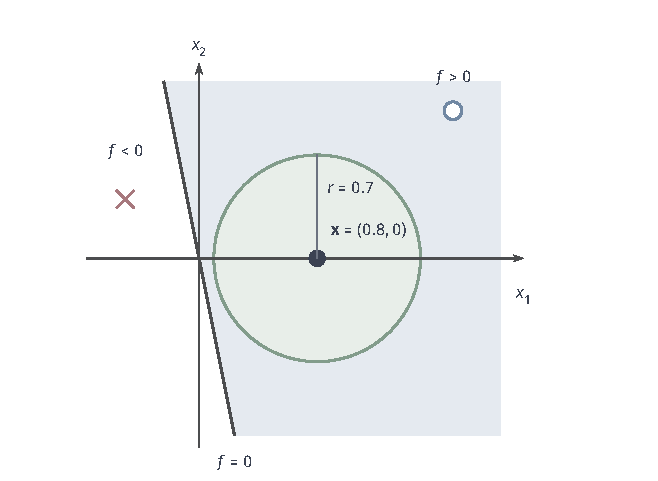
\includegraphics[width=111.404mm]{figures/06-foundations/03-trustworthiness/tikz/trust-certified-region/figure.pdf}
  \caption{教学分数$f(\bm x)=x_1+0.2x_2$在$(0.8,0)$取0.8，$L=\sqrt{1.04}$，$r=0.7$满足$0.8>Lr$，故闭球内符号正。深线为零边界，球外空心点正、叉点负；球外不受这份证书判定。证书保证符号保持，未判原标签正确。}
  \label{fig:trust-certified-region}
\end{figure}

对深度网络，直接估计的 Lipschitz 常数往往很大，由它得到的认证半径小到没有用处。于是出现了另一条思路：不直接给原分类器发证，而是先构造一个便于认证的新分类器，再给新分类器发证。\term{随机平滑}（randomized smoothing）是代表：在原分类器$h$的输入上注入高斯噪声，对噪声下的预测投票，以得票概率最高的类别作为新分类器$g$的输出，平局按预先固定的规则裁决：
\begin{equation}
 g(\bm{x})=\arg\max_k
   \mathbb P_{\bm{\varepsilon}\sim
   \mathcal N(\bm{0},\sigma^2\bm I)}
   \{h(\bm{x}+\bm{\varepsilon})=k\}.
 \label{eq:robustness-smoothing}
\end{equation}
其中$\bm{x}\in\mathbb R^d$，$\bm I$是$d$阶单位阵，$\sigma>0$是噪声的标准差。直觉是：输入发生小变化时，以$\bm x$为中心的噪声云团只是轻微平移，各类的得票概率随之平缓变化，而这种变化可以用高斯分布精确控制；可认证性来自噪声带来的平滑，不依赖原模型$h$的形状。Cohen 等利用两个平移后高斯分布之间概率质量的关系，为平滑分类器$g$建立了$\ell_2$扰动下的证书\scite{cohen2019smoothing}。认证对象始终是新规则$g$，不是原模型$h$。

记$\underline p_a\in[0,1]$为胜出类别$a$的投票概率下界，$\overline p_b\in[0,1]$为其他每个类别投票概率的共同上界。当$\underline p_a>\overline p_b$时，类别$a$在任何满足下式的扰动$\bm\delta$下都保持胜出：
\begin{equation}
 \lVert\bm{\delta}\rVert_2<r_{\mathrm{cert}},
 \qquad
 r_{\mathrm{cert}}
 =\frac{\sigma}{2}
 \left[\Phi^{-1}(\underline p_a)
       -\Phi^{-1}(\overline p_b)\right]
 \label{eq:robustness-smoothing-radius}
\end{equation}
其中$\Phi$是标准正态分布函数，$\Phi^{-1}$是其分位函数，端点0和1按极限理解。$\Phi^{-1}$把概率换算成“标准差个数”：$\Phi^{-1}(0.5)=0$，$\Phi^{-1}(0.9)\approx1.28$。式中括号内是胜出类与其他类之间的票数差距在这种尺度下的长度，乘以$\sigma/2$换算回输入空间的距离。票差越大、噪声尺度越大，半径就越大。二分类时有一个可以直接验证的特例：若原分类器$h$是一个半空间，即$\bm x$离决策超平面的距离为$s$且位于类别$a$一侧，则噪声沿超平面法向的分量服从$\mathcal N(0,\sigma^2)$，$h(\bm x+\bm\varepsilon)=a$的概率恰为$p_a=\Phi(s/\sigma)$。取$\overline p_b=1-p_a$，由$\Phi^{-1}(1-p)=-\Phi^{-1}(p)$，式中半径化为$\sigma\Phi^{-1}(p_a)=s$，正好是到边界的距离。对一般的$h$，Cohen 等的证明表明：在$\bm x$处得票概率相同的所有分类器中，半空间是输入平移后得票下降最快的情形，因此同一半径对一般的$h$也成立。这个半径保证的是投票规则：半径内任意扰动下，平滑分类器的输出都是$a$；它既不保证某一次带噪声的$h$预测正确，也没有给原模型发证。

实际中投票概率未知，只能用蒙特卡洛抽样估计，并用有效的置信界把抽样误差计入证书。看一个量级：二分类时其他类只有一个，若已知$\underline p_a=0.9$，则对方的概率至多$0.1$，可令$\overline p_b=0.1$。取$\sigma=0.25$，由$\Phi^{-1}(0.1)=-\Phi^{-1}(0.9)$得认证半径
\[
 \frac{0.25}{2}[\Phi^{-1}(0.9)-\Phi^{-1}(0.1)]=0.25\,\Phi^{-1}(0.9)\approx0.25\times1.282\approx0.32.
\]
这里的0.9必须是有置信保证的下界，90\%的经验票数不能直接当作0.9。还有一个选择偏差要处理：用同一批样本既选出胜出类别、又估计该类概率会使界失效，必须为选类和估概率分别独立采样，或采用对选择同时有效的程序。抽样不足以把胜出类与其他类分开时，应拒绝认证，而不是硬给一个半径。

增大$\sigma$并不一定让证书更实用。$\sigma$在式中是乘性因子，但改变噪声也会改变各类投票概率：更强的噪声可能缩小胜出类与其他类的概率间隔，也可能损害分类正确率，二者没有一般的单调规律。因此不能固定概率界、只看$\sigma$就断言半径变大，而须重新估票、认证并评价准确率。平滑还要为每个输入做多次前向计算，成本显著增加。

有了逐样本证书后，可以汇总成总体指标。给定目标半径$r$，对每个样本检查两件事是否同时成立：预测正确，且认证半径不小于$r$；满足的样本占比就是该半径下的\emph{认证准确率}。报告时至少要给出认证准确率随半径变化的曲线、计算成本和认证失败的比例。也可以把搜索与认证并列，报告搜索鲁棒准确率：搜索找到反例则判该样本失败，证书成功覆盖则判稳定，两者都没有结论时保留“未判定”，不强行归类。两点统计边界要记住：单样本证书的置信界不自动保护整批样本或整条曲线，对整批下联合结论要为每个点分配失败概率；逐点证书也不保证测试样本代表未来总体，要升级为总体风险结论，仍需回到抽样条件。这里的随机性来自估票抽样，与上一章共形覆盖所依赖的“校准样本加新样本”的随机性是不同对象。

\subsection{变化识别与拒绝效果的检验}
\label{sec:robustness-monitor-test}

风险测试和邻域认证都只覆盖事先声明的范围。输入落到范围之外时，另一条防线是让系统识别出来并报警、转交人工，从而限制模型的使用。这里要分开检验两件事：识别“输入已离开熟悉范围”的能力，以及识别之后实际损失降低了多少。这两项证据支持的是系统层面的止损，并不证明分类器在这些输入上仍然正确——拒绝往往意味着承认模型在这里不可靠。

\term{分布外检测}（out-of-distribution detection，简称 OOD 检测）要判断一个输入是否来自训练分布之外。这句话要变得可检验，先得固定三个参照物：域内分布是什么、检测的输入单位是什么（一封邮件、一张图还是一个会话）、“域外”由哪些备择来源代表。“域外”本身也不是单一对象：训练时没见过的语义新类别、输入边缘分布改变的协变量变化、以及域内本就罕见的低密度样本，是三种不同情况。实验里某个域外数据集只代表那一个选定来源，不代表一切未知。

检测通常先给每个输入算一个异常分数，再选阈值：分数高于阈值就判为域外。分数可以是输入表示到训练集最近邻的距离，也可以是密度估计的负对数，或由分类器输出构造（第~\ref{sec:robustness-rejection}节）。例如，一封邮件的表示离所有训练邮件都很远，距离分数就高。这里有两个直觉错误要避免：低密度不等于难预测，罕见但规则明确的输入可能很好分；高置信也不等于熟悉，模型可以对陌生输入自信地出错。仅凭有限的参考数据，也不可能识别任意形式的未知分布。

检验流程上，先固定异常分数的定义，再分别保留三份数据：域内资料、预先指定的未知类别或来源，以及一份独立的验证集用来选阈值；最后在测试集上报告两类错误——误拒正常输入的比例和误接纳未知输入的比例。ROC 等排序曲线适合比较不同分数的整体区分力，但选定工作点时要结合两种错误的具体成本，曲线下面积本身没有计入成本。FPR95 这类指标还要核对方向和分母：若把域内定义为正类，FPR95 表示保留95\%域内输入时域外输入被错误接纳的比例，引用前必须确认它说的是哪一侧。

识别准确不等于止损有效：熟悉的输入也可能分错，陌生的输入也可能恰好分对。要评价拒绝是否减少了损失，须另取任务标签，计算上一章定义的接受风险、总体处理比例和转交成本，并在相同处理量或相同成本下比较不同规则。这样，第~\ref{chap:trust-reliability}章的选择性预测检验就与检测接了起来：域外标签检验“陌生的能否被识别”，任务标签检验“拒绝之后错误是否真的下降”。第~\ref{sec:robustness-rejection}节还会具体构造检测分数。

分布外检测针对单个输入是否陌生，\term{漂移检测}（drift detection）则针对一段数据流：观察数据的统计关系是否随时间改变。典型做法是取一个参考时间窗（如模型上线前一个月）和一个当前窗，比较两窗中某些统计量，例如模板甲的占比、输入特征的分布或模型预测为垃圾邮件的比例，用双样本检验判断差异是否超出抽样波动。检验的对象决定了它能发现什么：比较输入特征只能发现输入分布的改变。输入分布改变与风险改变之间没有必然联系。模板占比的改变很容易被输入特征的统计检验发现，但模型若本来不靠模板分类，风险未必增加；反过来，发件主体被接管时，输入的边缘分布几乎不变（还是那些地址、那些措辞），标签关系却已改变，纯输入漂移检测可能毫无反应。因此在缺少标签时，漂移信号只能作为“启动调查或暂时收窄使用”的触发器，不能决定模型往哪个方向更新；要把输入信号与真实错误对应起来，仍需持续获得少量真实标签。反复查看同一批监测数据挑出来的“漂移点”，也不能直接套用为固定一次检验设计的区间。

评价报警机制时应保留时间顺序，把已知无变化和有变化的时间段分开，分别测量误报率、漏报率和发现延迟，并保存窗口长度、阈值和重置规则，结果才可复现。真实部署中变化起点通常未知，此时只能报告已核实的统计差异及差异出现后的风险，不能把所有报警都算作真阳性。等延迟返回的标签补齐真实风险后，再另行核算“因报警而拒绝或更新”带来的收益和代价。

\section{鲁棒性的增强}
\label{sec:robustness-enhancement}

增强方法的选择应由诊断决定。对应前面的失效机制：标签保持的局部错误，需要约束模型对输入变化的行为；困难群体被平均目标忽略或环境中存在捷径，需要调整训练风险和所依赖的依据；范围外输入信息不足，需要拒绝；新环境确实带来了可用信息时，才考虑让模型适应。前三类措施不要求在部署中持续改变模型参数；适应则要额外处理状态更新、错误累积和旧能力遗忘。这些措施可以组合，但评价时要分清各自改变了什么。

动手之前先排除一个平行问题：数据污染。个别标注错误或测量异常会产生极大的残差，在平方损失下，单个点对梯度的贡献随残差线性增长，可以把模型拉向错误方向。Huber 损失（Huber loss）在残差$r$的绝对值不超过阈值$c$时使用平方项$r^2/2$，超过后改为线性项$c|r|-c^2/2$（两段在$|r|=c$处值与导数都衔接）。它对残差的导数被截在$[-c,c]$内，于是每个点对梯度的贡献最多为$c$量级，单个异常点的影响被截断；其他稳健损失或迭代降权也有类似作用。但机械降权有一个风险：合法的少数群体在训练数据中代表不足，残差也可能天然较大，把它们当噪声压下去会进一步牺牲这些群体。因此异常标签、测量噪声与“模型还没学会的合法样本”要靠数据诊断区分，不能只凭残差大小处理。

\subsection{输入变化下的行为约束}
\label{sec:robustness-local-enhancement}

最直接的思路，是把任务预期的标签保持变换$T$（如压缩、改写）放进训练，用$\ell(f(T(\bm{x})),y)$要求模型对变换后的输入仍预测原标签。没有标签时（如无监督一致性训练），可以改为约束变换前后的概率、分数或中间表示彼此接近，并明确用什么量衡量差异、权重多大。前提是变换真的保留任务含义：一致性约束加得过强，会把有意义的差异也强行抹掉，例如把“否定词被删”这种改变语义的变化也当成应当保持。

除了约束同一样本变换前后的预测，还可以约束不同样本之间预测怎样过渡。\term{混合增强}（mixup）用同一个权重对两个输入和它们的标签分别做线性插值。设$\bm{e}_y$为类别$y$的独热标签，则混合样本和混合标签为
\begin{equation}
 \begin{aligned}
  \widetilde{\bm{x}}&=\lambda\bm{x}_i+(1-\lambda)\bm{x}_j,\\
  \widetilde{\bm{y}}&=\lambda\bm{e}_{y_i}
                         +(1-\lambda)\bm{e}_{y_j},
 \end{aligned}
 \label{eq:robustness-mixup}
\end{equation}
其中$\lambda\in[0,1]$是输入和标签共用的插值权重，通常从对称的 Beta 分布中随机抽取。用软标签交叉熵训练时，两类的损失按$\lambda$和$1-\lambda$的比例分担，并不强迫这个“介于两者之间”的样本属于某个端点类别\scite{zhang2018mixup}。

当两个端点类别不同时，例如$\lambda=0.7$，混合标签就是两类上的概率向量$(0.7,0.3)$：模型看到70\%甲样本与30\%乙样本混合而成的输入时，输出也应接近这个向量。这在样本之间加了一条平滑过渡的约束，但它依赖一个语义假设：插值出来的点是有意义的。两张图按像素混合通常还能看出内容；两封邮件按字节混合往往只是乱码，在表示空间插值是否合理也需要单独核验。端点标签正确也不证明中间的软标签就是真实标签分布，因此 mixup 约束的对象与式~\eqref{eq:robustness-perturbation-risk}的“标签保持邻域”不同。

AugMix 走的是另一条路：从同一张图像出发生成多条随机增强链，把这些视图混合起来并保留原图通路，还可以训练模型对各视图给出一致预测\scite{hendrycks2020augmix}。它约束的是“同一对象在合理变化下的表现应当一致”，不规定不同类别之间存在线性过渡。两种方法的假设由此分开：mixup 比较不同样本之间的过渡，AugMix 比较同一样本的多个合理视图，不能笼统地说“增强数据就更鲁棒”。增强前要检查小目标、关键颜色或文字方向有没有被破坏；增强后要用训练时没有用过的损坏类型及其组合复查，否则测到的只是对所选增强的拟合。

随机增强还有一个覆盖问题：随机抽到的大多是“容易”的变化，可能恰好漏掉允许邻域中少数让模型严重出错的位置，而这些位置正是式~\eqref{eq:robustness-perturbation-risk}中上确界关心的。最不利训练主动去寻找这些高损失位置并在那里施加压力。要设计这样的目标，先看鲁棒零一错误由什么组成：一个样本鲁棒地出错，是指允许邻域内存在分错的变体。这可以拆成两种互斥情形——原输入已经分错；或原输入分对，但邻域内存在分错的变体。前者需要改善干净输入上的分类，后者需要让决策边界远离样本。TRADES 的理论分析通过分类校准损失及相应转换，把这两部分分别与可优化的代理量联系起来\scite{zhang2019trades}。

令$\bm{p}_{\bm{\theta}}(\bm{x})$表示模型输出的类别概率向量，$p_{\bm\theta,y}(\bm x)$为其中类别$y$的分量，$\bm{\theta}$为参数向量、$\Theta$为候选参数集，$\mathcal P_{\mathrm{train}}$为训练数据的联合分布。TRADES 对两种情形各设一项：
\begin{equation}
 \begin{aligned}
 \min_{\bm{\theta}\in\Theta}\
 \mathbb E_{(\bm{x},y)\sim\mathcal P_{\mathrm{train}}}
 \bigg[&-\log p_{\bm{\theta},y}(\bm{x})\\
 &+\beta\sup_{\bm{x}'\in U(\bm{x})}
 D_{\mathrm{KL}}\!\left(
 \bm{p}_{\bm{\theta}}(\bm{x})
 \,\middle\|\,
 \bm{p}_{\bm{\theta}}(\bm{x}')\right)\bigg],
 \end{aligned}
 \label{eq:robustness-trades}
\end{equation}
其中$D_{\mathrm{KL}}(\bm p\,\|\,\bm p')=\sum_kp_k\log(p_k/p'_k)$是 KL 散度，衡量两个类别分布的差异，非负且仅在两者相同时为0；$\beta>0$控制稳定性项相对于分类项的权重，外层期望在实现时用样本平均近似。第一项是干净输入上的负对数似然，把真实类别的概率抬高，对应“原输入分错”的情形；第二项惩罚邻域内预测分布的最大变化，对应“邻域内会翻转”的情形，而且专门盯住最容易被扰动改变预测的位置。如果去掉分类项、只保留稳定项，对所有输入输出同一分布就能让 KL 为零，却完全不区分类别，这说明两项缺一不可。

读这个目标要注意两层近似。第一，内层上确界通常只能用有限步梯度搜索近似，找到的是偏离的一个下界，而非全局最坏点。第二，交叉熵加 KL 是沿理论动机构造的训练代理，其数值不能直接解释为鲁棒零一风险的上界：原论文的风险界还包含校准转换、最优自然风险与最优代理风险等量；从代理下降到风险受控，仍须核对损失条件、推广误差和内层求解误差。

训练前还要核验邻域定义本身是否自洽。如果两个不同类别的样本在规定邻域内互相重叠，同一个点就会被要求同时属于两类，这种矛盾不能靠调大$\beta$解决。确认范围相容后再选择$\beta$；内层搜索仍会增加训练计算。对抗扰动的搜索与梯度遮蔽等更细致的检验留到第~\ref{chap:trust-security}章。

图~\ref{fig:trust-adversarial-training-loops}把式~\eqref{eq:robustness-trades}的内外两层拆开：内层固定参数，在邻域$U(\bm x)$中寻找使原预测与扰动预测 KL 散度最大的扰动；外层用干净输入的分类损失加加权的 KL 项更新参数，随后重新搜索，内外交替进行。内层产生的只是“当前找到的最坏候选”。

\begin{figure*}[htbp]
  \centering
  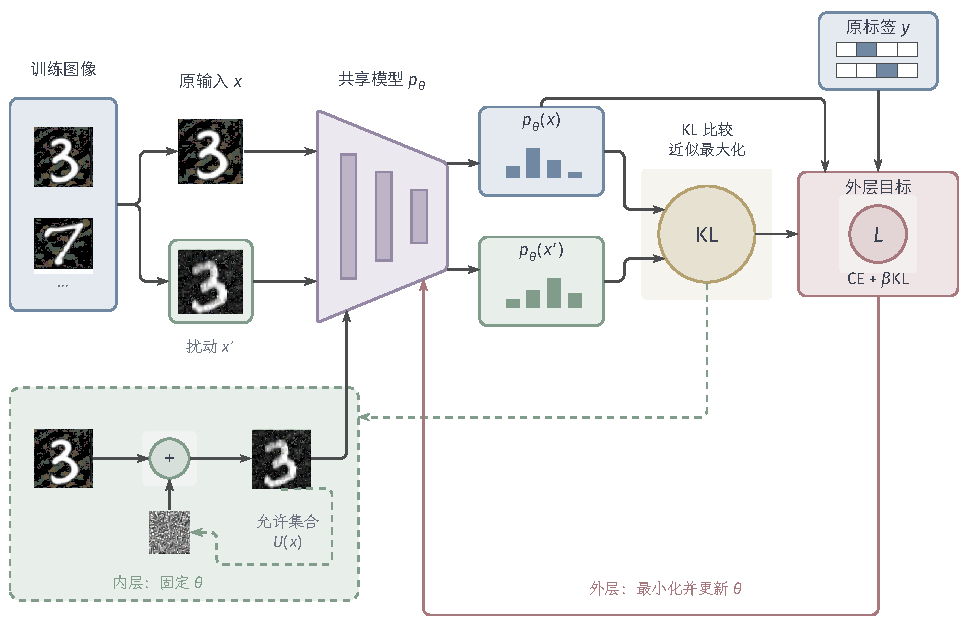
\includegraphics[width=164.600mm]{figures/06-foundations/03-trustworthiness/tikz/adversarial-training/figure.pdf}
  \caption{TRADES内层固定参数，在$U(\bm x)$近似增大原、扰动预测之间的KL；外层最小化原输入的分类损失与加权KL，再重新搜索。共享模型分别处理两输入，原预测还独立进入分类损失。数字样本和箭头均为示意，未提供实际扰动大小或全邻域形式证书。}
  \label{fig:trust-adversarial-training-loops}
\end{figure*}

鲁棒性常被说成“免费”，也常被说成必然牺牲准确率。图~\ref{fig:trust-robust-accuracy-tradeoff}用一个固定样本和扰动的教学比较说明两种说法都不完整。这里的鲁棒正确指原输入分对、且搜索在邻域内没有找到分错的变体，所以鲁棒正确的样本是干净正确样本的子集。四个候选模型中，A、B、C 的干净正确数依次升高（80、88、94），鲁棒正确数却依次下降（70、60、45），呈现取舍；但 D 干净90、鲁棒74，两项都优于 B。因此虚线只连接 A、B、C 以展示一种可能的取舍，不是所有任务上都成立的最优边界；是否存在真实取舍，必须在固定样本、固定邻域和搜索条件下比较。

\begin{figure*}[htbp]
  \centering
  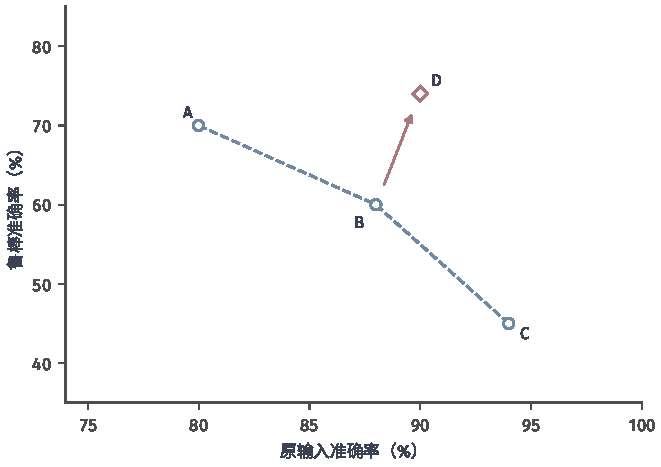
\includegraphics[width=112.000mm]{figures/06-foundations/03-trustworthiness/matplotlib/trust-robust-accuracy-tradeoff/figure.pdf}
  \caption{固定100个教学样本和标签保持邻域，原输入、鲁棒正确数依次为A 80/70、B 88/60、C 94/45、D 90/74。鲁棒正确是原正确子集，D两项优于B。虚线仅连A、B、C，不是实验或普遍最优边界；比较还需共同扰动及搜索条件。}
  \label{fig:trust-robust-accuracy-tradeoff}
\end{figure*}

改变训练约束后，仍要按第~\ref{sec:robustness-risk-test}节在独立数据上测试；若声称严格的邻域稳定，则要另用第~\ref{sec:robustness-certification}节的认证。训练目标降得再低，也不能直接推出证书半径变大——前者是经验优化量，后者是形式化保证。

\subsection{跨环境风险与稳定依据的约束}
\label{sec:robustness-environment-enhancement}

局部邻域约束既没有改变不同环境在训练中的权重，也没有判断模型依赖的依据能否跨环境成立。当问题出在困难群体被平均目标忽略、或预测关系随环境变化时，需要换一个层次：损失定义不变，但扩大训练目标所覆盖的环境，并明确希望模型依赖的、跨环境保持的预测关系是什么。

普通训练最小化参考分布上的平均风险；如果担心部署分布会在某个范围内变动，自然的做法是让模型在这个范围内最差的分布上也表现尚可。先按任务规定一个允许分布族$\mathfrak Q$：例如允许已声明的各环境以任意比例混合，或允许真实分布在参考分布周围某个预设距离内变化。\term{分布鲁棒优化}（distributionally robust optimization, DRO）比较每个候选模型在族内最坏分布下的风险，从模型族$\mathcal F$中选出把这个最坏风险压得最低的模型。监督学习下的目标为
\begin{equation}
 \min_{f\in\mathcal F}\ \sup_{\mathcal Q\in\mathfrak Q}
   \mathbb E_{\mathcal Q}\ell(f(\bm{x}),y).
 \label{eq:robustness-dro}
\end{equation}
读法是由内向外：内层对固定的$f$找出族内期望损失最高的分布，得到$f$的“最坏成绩”；外层在模型族里挑最坏成绩最好的模型。这是一个极小极大结构，可参考\BookChapterRef{chap:decision-theory-and-dynamic-risk}{卷2《数学准备：概率、因果与决策》第6章“策略的价值与优化”}。

DRO 首先是一个训练或压力测试目标：用它训出的模型仍须独立测试，目标值本身不给部署提供证书。若想得到高概率的风险上界，还需要额外的统计构造：从训练集$S=\{(\bm{x}_i,y_i)\}_{i=1}^n$出发构造数据驱动的不确定集合$\widehat{\mathfrak Q}(S)$，用独立资料或预先固定的统计规则选择距离、半径或分组，并证明真实分布以至少$1-\delta$的概率落在$\widehat{\mathfrak Q}(S)$内；再把这层包含关系与推广误差、内层上确界的近似误差合在一起，才能转成最终风险界。集合设得太小会漏掉真实变化，设得太大又会包含无意义的压力情形，使模型过于保守。

在一种重要的特殊情形下，DRO 化为很直观的形式。设共有$G$个组，组$g$的分布为$\mathcal P_g$，组内风险为$R_g(f)=\mathbb E_{\mathcal P_g}\ell(f(\bm{x}),y)$。若允许分布族就是这些组按任意比例$\bm q=(q_1,\ldots,q_G)$的混合，则混合分布下的风险是各组风险的加权和$\sum_gq_gR_g(f)$，比例$\bm q$取遍概率单纯形$\Delta_G=\{\bm q\in\mathbb R^G:q_g\geq0,\ \sum_gq_g=1\}$。此时
\begin{equation}
 \sup_{\bm{q}\in\Delta_G}\sum_{g=1}^{G}q_gR_g(f)
       =\max_{1\leq g\leq G}R_g(f).
 \label{eq:robustness-group-dro}
\end{equation}
理由分两步：任一加权平均都不超过其中的最大项，即$\sum_gq_gR_g\leq\sum_gq_g\max_{g'}R_{g'}=\max_{g'}R_{g'}$；而把全部权重放到风险最高的组，等号就取到。于是式~\eqref{eq:robustness-dro}退化为“最大组风险最小化”，称为组 DRO。在示例~\ref{ex:robustness-mixture}中，普通平均目标主要由占99\%的常见模板决定，少见模板几乎没有话语权；最大组目标则首先盯住少见模板那50\%的错误率。

组 DRO 能防止大组的低风险在平均中压过小组的高风险，但不消除组内自身的泛化误差。Sagawa 等指出，过参数模型可以把所有训练组的误差都拟合到零，此时训练上的最坏组风险也为零，最坏组在新数据上的表现仍需配合更强的正则和专门的验证\scite{sagawa2020groupdro}。计算上可以交替进行：增大当前高损失组的权重，再更新模型。若担心“任意比例”过于保守，也可以只允许混合比例在当前比例附近变动。

实际使用组 DRO 有三个问题。分组太粗会漏掉组内的捷径，太细又使每组样本太少、估计剧烈波动；组标签本身未必总能拿到；若按“哪些样本损失高”自动分组，还容易把标注错误样本混进“困难组”，而优化目标本身分不清高损失样本是合法的困难群体还是脏数据。另外，把各组风险都压低并不等于机会或成本的分配是公平的：各组错误率相等也可能只是“一样地差”，同样的错误对不同组的后果也可能不同。第~\ref{chap:trust-fairness}章会先确定分配原则，再判断哪些差异有意义；组 DRO 只在既定损失和分组上做优化，不能据此声称模型公平。

多个环境还有另一种价值：帮助识别跨环境稳定的依据。直觉是，如果某条关系在所有环境中都成立，它更可能是可迁移的。不变风险最小化（invariant risk minimization, IRM）沿着这个思路，寻找一种特征表示，使同一个预测规则在所有训练环境上都同时最优；组 DRO 则只约束最坏组的损失，不要求各组的最优规则一致。两者都可能被“同向捷径”骗过：如果所有训练环境中模板与标签都同向相关，模板在各环境中也是“不变的”，IRM 同样可能依赖它。反过来，若各环境的真实最优规则本来就不同，强迫共用一条规则会丢失合理的环境特异信息。从不变性到目标域保证所需的条件见第~\ref{sec:domain-generalization}节；仅凭多个训练环境上的表现一致，不能保证在任意新环境成立。

评价这些目标时，比较条件必须对等。DomainBed 在七个多域数据集上用统一实现比较了九种方法和三类模型选择准则，报告普通经验风险最小化（ERM）在这些设置下取得了当时领先的目标域准确率\scite{gulrajani2021}。这说明方法名称带来的直觉不能替代相同条件下的认真比较，调参充分的简单基线往往很强；反过来，这一结论也只限于它比较过的数据集和设置，不能说 ERM 在一切变化下都最优。要把收益归因到训练目标，应固定架构、训练预算、增强方式和可见的验证环境，只改变目标本身。第~\ref{chap:transfer-learning-theory}章回答“信息何时足以识别可迁移规律”，受控实验检查具体算法是否有效利用了这些信息，两者缺一不可。

\subsection{超出适用范围时的拒绝策略}
\label{sec:robustness-rejection}

当数据中的信息不足以覆盖所有可能输入时，再怎么训练也无法对域外输入作出可靠承诺。这时现实的做法是提高接纳条件：只在模型足够有把握时自动给出预测，否则交给人工。拒绝增强的是系统的变化应对能力，不是被拒输入上原模型的准确性：它只是不再自动执行这部分决定，被拒输入也可能恰好能被分对。拒绝的理由应是证据、风险容限或适用范围；报告时把处理量的减少和人工负担的增加与模型质量的收益分开记录。

拒绝需要一个“熟悉程度”分数。最简单的是\term{最大类别概率}（maximum softmax probability, MSP）：取 softmax 输出中的最大概率，低于阈值就拒绝。Hendrycks 与 Gimpel 把它作为错误样本和分布外样本检测的基线，好处是无需重新训练模型\scite{hendrycks2017msp}。

MSP 的弱点在于 softmax 只看类别分数之间的差。设模型对$K$个类别输出未归一化分数（logits）$z_1,\ldots,z_K$，softmax 概率为$\exp(z_k)/\sum_j\exp(z_j)$。给所有$z_k$加同一个常数$c$，分子分母同乘$e^{c}$，概率不变。看一个构造：两个输入的 logits 分别为$(10,9)$和$(1,0)$，前者是后者每项加9，所以 softmax 之后最大概率同为$e/(e+1)\approx0.731$，MSP 给它们相同的熟悉分数。logits 的整体幅度信息在归一化时被丢掉了。

若想保留这项幅度信息，可以从$K$个类别的实值分数$z_k(\bm{x})$和温度$T>0$构造\term{能量分数}（energy score）：
\begin{equation}
 E_T(\bm{x})=-T\log\sum_{k=1}^{K}
       \exp\!\left(\frac{z_k(\bm{x})}{T}\right).
 \label{eq:robustness-energy}
\end{equation}
它可以理解为“取负的平滑最大值”：由$\exp(\max_kz_k/T)\leq\sum_k\exp(z_k/T)\leq K\exp(\max_kz_k/T)$，有$\max_kz_k\leq-E_T(\bm x)\leq\max_kz_k+T\log K$。所以最大 logit 越大，能量越低；常把较大的能量作为域外信号。在$T=1$时，前面两个向量的能量分别约为$-(10+\log(1+e^{-1}))\approx-10.313$和$-1.313$，MSP 无法区分的两点现在可以区分。能量的符号和范围随 logits 的公共偏移改变，并不总是负数，“更大”也不等于“更接近0”，阈值与方向应由独立验证记录确定。Liu 等比较了直接用能量检测，以及在训练中显式拉开域内与域外输入能量的方案\scite{liu2020energy}。

能区分这两个点，不等于能量高低对应“陌生的程度”。给所有类别的分数加上同一个与输入有关的常数，会改变能量却不改变 softmax 概率，因而也不改变交叉熵训练目标。这说明分类训练本身并不确定这项公共幅度，能量不是输入的对数密度，除非另做生成式拟合。因此能量阈值须在实际模型和实际备择数据上验证。

如果能获得一批辅助的异常数据，还可以用\term{异常暴露}（outlier exposure, OE）让模型在训练时就“见过异常”：在正常任务损失之外，增加一项对任务外输入的约束。一种分类实现是让模型对异常输入输出接近均匀的分布，避免它对陌生样本也给出尖锐的类别判断\scite{hendrycks2019oe}。

异常暴露的限制是：辅助异常不可能代表全部未知来源；如果同一批异常数据既用于训练又用于测试，模型可能只学会识别这批数据的来源线索。应留出训练时没见过的异常类别和来源，并在测试前固定好各组。对邮件任务，可以把从未见过的诈骗模板来源作为“与域内较相似”的备择，把非邮件文档（如纯文本表格）作为“差异明显”的备择；这两组都只是预先选定的检验来源，不构成对未知的完备覆盖。按第~\ref{sec:robustness-monitor-test}节冻结阈值、独立检验后，应分别报告各组输入被误接纳的比例。

\subsection{利用新环境信息时的风险与验收}
\label{sec:robustness-adaptation}

前三类增强都不要求模型在部署中改变自己。最后一类不同：新环境不断产生数据，模型可以利用这些数据在线改变运行状态，例如用新数据重新估计网络中批归一化层的均值和方差（新相机使图像整体变暗时，这些统计量会随之改变）、做部分参数更新，或把当前模型的高置信预测当作\term{伪标签}（pseudo-label）反过来参与训练。\term{测试时适应}（test-time adaptation）是这类方法的统称：模型在测试阶段、通常没有真实标签的情况下根据新输入调整自身。具体算法可参考\BookChapterRef{chap:ket-transfer-adaptation}{卷8《学习范式：知识的获取、演进与迁移》第13章“知识的迁移”}，本节只检查它怎样改变可靠性主张，以及验收需要什么条件。

无标签适应最大的风险是更新方向只能依赖代理信号，如预测置信度、增强前后预测的一致性。代理改善不等于任务风险下降：模型可能把自己的错误预测通过高置信伪标签不断强化（自证循环），也可能因为对所有输入都输出常数而显得“一致性很好”。限制可更新的参数范围、步长和每批样本数量，可以缩小出错时的影响范围，但不能证明更新方向正确。只要能拿到少量真实标签，就应优先用它核验任务表现。

适应模型还有一个离线评估容易忽略的特点：它的输出依赖自身状态，而状态由处理历史决定。批次如何划分、样本以什么顺序到达、对一个输入先预测还是先更新、何时重置状态，都会使相同的输入在不同时刻面对不同的模型，这些都属于必须明确的程序定义。把数据顺序打乱后做离线适应，不能代表时间相关的真实服务；只评价发生了高置信更新的那部分样本，也会遗漏其余输入和困难群体。

因此评价适应程序时，应让冻结的对照模型与适应模型在同一条时间流、同样的计算预算下并行运行，报告两者在新旧环境上的风险、风险随时间的轨迹、关键组表现、回退是否有效，以及更新和状态保存的成本。部署前还要写死一组规则：新环境的风险容限；相对冻结参照，旧环境和关键组的风险最多允许增加多少；连续几个时间窗越界就触发动作；回退到哪个版本；用什么资料复验。总体平均收益不能抵消某个短时间窗的严重退化，新环境的收益也不能掩盖旧能力的遗忘，这两条都要由预设规则约束，不能事后解释。

标签不足以判断更新方向时，稳妥的处置是保留冻结参照、收窄自动处理范围或回退，避免模型沿错误的代理信号继续优化；这些处置只是止损，不证明适应成功。只有把模型版本、更新规则、运行状态和验收条件全部固定下来，观察到的结果才能归因于完整的适应程序，而不是某个偶然的状态轨迹。

\section{本章小结}
\label{sec:robustness-summary}

本章把两类问题分开：变化之后模型本身的表现如何，以及证据不足时系统怎样止损。变化有三个层次——输入测量扰动、群体比例改变、特征与标签规律改变；典型失效机制是决策边界过近、困难组占比上升与捷径依据失效。二者不是一一对应的，明确实际路径后才能选择补救。检验上，受控损坏基准和跨来源测试回答平均风险，局部证书回答指定邻域内不翻转，分布外检测、漂移监测、拒绝和回退回答范围外能否止损；它们的证据对象不同，不能互相替代。

增强方法按改变的对象区分：数据增强与局部稳定训练约束模型对输入变化的行为，分布鲁棒优化（包括最大组风险）改变训练风险对环境和群体的加权，范围外拒绝不改变模型而只收窄它的自动决定权，测试时适应用新环境信息更新运行状态，同时承担错误自我强化和旧能力遗忘的风险。无论哪种方法，都要与调优充分的基线比较，并同时检查原环境、新环境、关键组与资源代价；证据不足时应收窄使用而不是强行部署。

回到开篇的误拦事故：先判断变化发生在测量、群体比例还是标签关系，再对应检查决策边界、原本就存在的高错误组和模型对模板的依赖，据此取得补救所需的信息。如果排查发现损失集中在某个人群，还要追问这种负担分配是否合理，这是下一章公平性要处理的问题；“模型究竟用了哪些因素作判断”，则由第~\ref{chap:trust-interpretability}章的解释方法回答。

\paragraph{扩展阅读}

常见损坏基准与WILDS分别提供受控扰动和真实来源差异的证据。对照阅读时保留类型、划分及模型选择条件，就能确定基准平均结果适用到哪里\scite{hendrycks2019corruptions,koh2021wilds}。

TRADES与组DRO分别针对局部稳定和最大组风险；测试时适应的状态、算法与实践仍需结合适应条件核查\scite{zhang2019trades,sagawa2020groupdro}。
